% vim: set filetype=tex

\section{\color{fancy}Chapter 1: Overview}
This chapter will give you a quick overview of common components as well as a short description of the software. Each component is explained in detail in their specific section, respectively.

\subsection{At A Glance}
\begin{figure}[h]
  \centering
  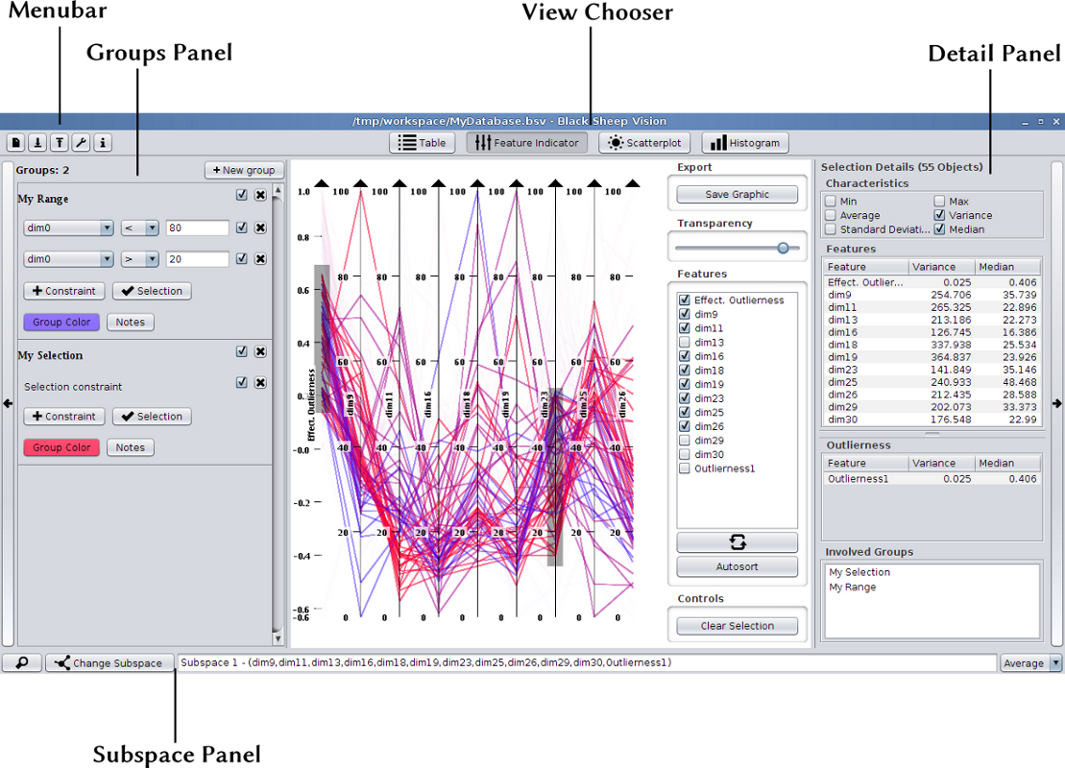
\includegraphics[width=12cm]{images/bsv/Overview.png}
  \caption{Overview}
  \label{fig:overview}
\end{figure}

\subsection{Description}
\begin{tabular}{p{0.2\linewidth}p{0.7\linewidth}}
  \color{fancy}Component & \color{fancy}Purpose \\ \hline
  Menubar & You can use the Menubar to create a new workspace, import your raw files, export data you worked on, adjust the settings or view a quick info dialog. \\ \hline
  View Chooser & By using the View Chooser, you are able to efficiently switch between different views. Due to the fact that all those views are representing your data in a unique way, you are able to improve the explanatory power of your data.  \\ \hline
  Groups Panel & The Groups Panel lets you structure your data by classifying and filtering it in the way you specify it, thus improving the vividness of your information. \\ \hline
  Detail View &  As soon as you have arranged your data, the Detail View shows you specific attributes concerning your selection. \\ \hline
  Subspace Panel & By using the Subspace Panel you are not only in control of the current subspace, but also are able to select the method, the effective outlierness is calculated by. \\ \hline
\end{tabular}
